\chapter{The sounds of English}\label{sounds}

\noindent For your convenience,\is{vowels|(} Figure \ref{fig:IPA-vowels} provides an overview of the different IPA symbols used for vowels. It also shows the positioning of these vowels in the vowel space. You will encounter 18 of these symbols throughout this book:

\begin{figure}[H]
%     \centering
%     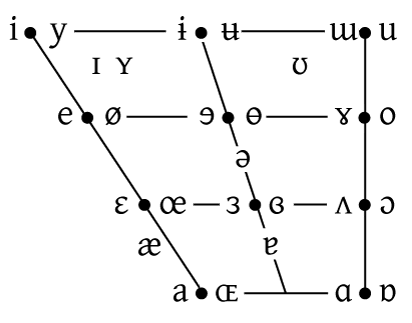
\includegraphics[scale=0.3]{chapters/img/IPA_vowel_symbols.png}
    \begin{vowel}
\putcvowel[l]{i}{1}
\putcvowel[r]{y}{1}
\putcvowel[l]{e}{2}
\putcvowel[r]{\o}{2}
\putcvowel[l]{\textepsilon}{3}
\putcvowel[r]{\oe}{3}
\putcvowel[l]{a}{4}
\putcvowel[r]{\textscoelig}{4}
\putcvowel[l]{\textscripta}{5}
\putcvowel[r]{\textturnscripta}{5}
\putcvowel[l]{\textturnv}{6}
\putcvowel[r]{\textopeno}{6}
\putcvowel[l]{\textramshorns}{7}
\putcvowel[r]{o}{7}
\putcvowel[l]{\textturnm}{8}
\putcvowel[r]{u}{8}
\putcvowel[l]{\textbari}{9}
\putcvowel[r]{\textbaru}{9}
\putcvowel[l]{\textreve}{10}
\putcvowel[r]{\textbaro}{10}
\putcvowel{\textschwa}{11}
\putcvowel[l]{\textrevepsilon}{12}
\putcvowel[r]{\textcloserevepsilon}{12}
\putcvowel{\textsci\ \textscy}{13}
\putcvowel{\textupsilon}{14}
\putcvowel{\textturna}{15}
\putcvowel{\ae}{16}
\end{vowel}

    \caption{IPA chart of cardinal vowels (Chart by Zieben007, licensed under CC BY-SA 4.0)}
    \label{fig:IPA-vowels}
\end{figure}

\noindent Similarly,\is{vowels|)} below we provide you with consonantal\is{consonants|(} IPA symbols that you will encounter as you read on.\medskip\\ 
\noindent
\fittable{\begin{tabular}{lllllllll}
\lsptoprule
~ & {Bi\-labial} & {Labio\-dental} & {Dental} & {Alve\-olar} & {Palatal} & {Velar} & {Uvular} & {Glottal} \\
\midrule
{plosives} & p, b &  & & t, d & & k, g & & ʔ \\
{fricatives} & & f, v & θ, ð & s, z & ʃ, ʒ & x & ʁ & h \\
{nasals} & m & & & n & & ŋ & & \\
{approximants} & ʍ, w & & & l, ɹ & & ʍ, w & & \\
{affricates} & & & & tʃ, dʒ & & & &  \\
{trills} & & & & r & & & ʀ & \\
{taps/flaps} & & & & ɾ & & & &  \\
{retroflexes} & & & & ɻ & & & &  \\
\lspbottomrule
\end{tabular}}\medskip\\
\noindent The approximants /ʍ/ and /w/ are labiovelar, which is why you can find them under both ``Bilabial'' and ``Velar'' columns.\is{consonants|)}
